\documentclass{beamer}
\usepackage{amsmath,amsfonts,amsthm,amssymb,chemformula,graphicx,multicol,multirow}
\usepackage[backend=biber,sorting=none,style=numeric-comp,giveninits]{biblatex}

\DeclareNameAlias{default}{family-given}
\renewbibmacro{in:}{}
\addbibresource{references.bib}

\usetheme{Madrid}

\usefonttheme{professionalfonts}

\newcommand{\vs}{\vspace{5mm}}

\title{Molecular Symmetry and Group Theory}
\author{Maggie Barker}
\institute[UNCW]{University of North Carolina Wilmington}
\date[Fall 2025]{December 8, 2025}

\begin{document}

    \frame{\titlepage}
    
    \begin{frame}{Introduction}
        Symmetry connects the world we see with the laws of chemistry. The language that describes symmetry is that of mathematics, in particular group theory, representation theory, and character theory. Countless chemical processes depend on symmetry, and an understanding of these concepts is rooted in algebra. We will take a interdisciplinary tour of this interface between chemistry and mathematics. Much of the presentation of point groups and character theory follows the treatments in \cite{miessler2014,mcgrady2024,vallance,young}.
        \vs

        \onslide<2>{
            We will:
            \begin{itemize}
                \item Introduce some basic chemistry principles to aid understanding
                \item Look at molecular symmetry and how to categorize it via point groups
                \item Discuss groups, matrices, and characters
                \item Build character tables for point groups from scratch
                \item Look at the interplay of symmetry and molecular vibrations
                \item Look at a few applications of character theory in chemistry
            \end{itemize}
        }
    \end{frame}

    \begin{frame}{Molecular bonding}
        Molecules are clusters of atoms that are bonded with one another by sharing pairs of electrons.
        \vs
    
        Two electrons shared between two atoms: Single bond (\ch{C-C}).
        
        Four electrons shared between two atoms: Double bond (\ch{C=C}).
        
        Six electrons shared between two atoms: Triple bond (\ch{C+C}).
        \vs
        
        Components of molecules can freely rotate along the axis of a single bond, but double and triple bonds are locked and cannot rotate.
    \end{frame}

    \begin{frame}{VSEPR theory}
        Molecular shape is determined by Valence Shell Electron Pair Repulsion theory (VSEPR). The name of the theory explains much of it:
        \vs
    
        \begin{itemize}
            \item Valence shell (outermost shell) electrons participate in bonding
    
            \item Electrons tend to occur in pairs
    
            \item Like charges repel, so electron pairs tend to be as far away from each other as possible
        \end{itemize}
        \vs
        
        Some electron pairs are bonding (shared with other atoms), and some will be nonbonding (not shared). A pair of nonbonding electrons is called a \emph{lone pair}.
    \end{frame}

    \begin{frame}{VSEPR Theory \cite{chemlearner}}
        \begin{center}
            \includegraphics[width=3in]{vsepr.jpg}
        \end{center}
    \end{frame}
    
    \begin{frame}{Molecular geometry}
        In water (\ch{H2O}), the oxygen atom is bonded to two hydrogen atoms and has two lone pairs. Hence, water is a bent molecule.
        \vs
    
        In ammonia (\ch{NH3}), the nitrogen atom is bonded to three hydrogen atoms and has one lone pair. Therefore, ammonia is a trigonal pyramidal molecule.
        \vs
    
        In methane (\ch{CH4}), the carbon atom is bonded to four hydrogen atoms and has no lone pairs. Thus, methane is a tetrahedral molecule.
    \end{frame}

    \begin{frame}{Polarity}
        If the atoms have similar electronegativity, the electrons will be shared equally, forming a nonpolar bond.
        \vs
        
        If one atom has higher electronegativity, it will attract electrons to it, causing the sharing to be unequal. This results in a polar bond.
        \vs
        
        If the polar bonds are equal and in opposite directions, they cancel by \emph{symmetry}, and the molecule will be \emph{nonpolar}. This occurs in carbon dioxide (\ch{CO2}), which is linear.
        \vs
        
        If the polar bonds do not cancel by symmetry, the molecule will be \emph{polar}. This occurs in water (\ch{H2O}), which is bent.
    \end{frame}

    \begin{frame}{Polarity of water}
        Many of the interesting characteristics of water are a direct consequence of hydrogen bonds, due to polarity.
        \vs
    
        If water were nonpolar, it would most likely be a gas at room temperature and behave more like carbon dioxide or methane. Life as we know it would be impossible if water was not a bent polar molecule!
    \end{frame}

    \begin{frame}{Symmetry elements and operations}
        Many molecules contain \emph{symmetry elements}, such as rotational axes, mirror planes, and inversion centers, upon which \emph{symmetry operations} can be performed. The molecule will be indistinguishable before and after the symmetry operation.
        \vs

        \onslide<2->{
            The most basic symmetry operation is $E$, the identity operation. This is the act of doing nothing, and is required in order to express a collection of symmetries as a group.
            \vs
        }

        \onslide<3>{
            A proper rotation, $C_n$, is a rotation that can be achieved in 3D space. It is a rotation through $360^\circ/n$ counterclockwise with respect to some axis. We have that $C_n^n\equiv E$, so $|C_n|=n$. If a molecule has more than one rotational axis, the one of highest order is called the \emph{principal axis}.
        }
    \end{frame}

    \begin{frame}{Symmetry elements and operations}
        A reflection over a mirror plane is denoted $\sigma$. In particular, a reflection plane that is perpendicular to the principal axis is called horizontal and denoted $\sigma_h$. A reflection plane that includes the principal axis is called vertical and denoted $\sigma_v$. A vertical reflection plane that bisects the angle between two $C_2$ axes is called dihedral and denoted $\sigma_d$.
        \vs

        \onslide<2->{
            The inversion operation, $i$, is where every point of the molecule is moved through the inversion center (the center of the molecule) to its opposite position the same distance from the center.
            \vs
        }

        \onslide<3>{
            An improper rotation, $S_n$, also called a rotation-reflection, is a $C_n$ rotation followed by a $\sigma_h$ reflection through a plane perpendicular to the rotation axis. Two $S_n$ operations together form a $C_{n/2}$ operation. An $S_2$ operation is equivalent to $i$. In some molecules, $S_j$ axes are coincident with $C_k$ axes.
        }
    \end{frame}

    \begin{frame}{Point groups}
        The collection of symmetry operations that a molecule possesses determines its \emph{point group}. It is named such since every symmetry element shares a single point. \cite{johnston2014}
        \vs
        
        There is a sequence of steps that can be followed to determine a point group.
        \vs
        
        To get started, we can classify molecules as being of \emph{low symmetry}, \emph{high symmetry}, or neither.
        \vs
        
        We will list the point groups of the three categories and show example molecules. To assist in the process, we will use a flowchart.
    \end{frame}
    
    \begin{frame}{Point groups of low symmetry}
        Molecules in the $C_1$ group have no symmetry besides $E$. (Indeed, every point group contains $E$, but it will be implicit.) (wedge-dash)

        \begin{center}\includegraphics[width=0.75in]{c1example.jpg}\end{center}

        \onslide<2->{
            Molecules in the $C_s$ group have only one mirror plane (in the following example, the mirror plane is the plane of the molecule).

            \begin{center}\includegraphics[width=0.75in]{csexample.jpg}\end{center}
        }

        \onslide<3>{
            Molecules in the $C_i$ group have only an inversion center.

            \begin{center}\includegraphics[width=0.75in]{ciexample.jpg}\end{center}
        }
    \end{frame}

    \begin{frame}{Point groups of high symmetry}
        Molecules in the $C_{\infty v}$ group are linear, with infinite rotation order and an infinite number of reflection planes containing the rotation axis. They contain no inversion center. An example is hydrogen chloride.

        \begin{center}\includegraphics[width=0.75in]{cinfvexample.jpg}\end{center}

        \onslide<2->{
            Molecules in the $D_{\infty h}$ group are like $C_{\infty v}$, but with perpendicular $C_2$ axes, a perpendicular mirror plane, and an inversion center. An example is carbon dioxide.

            \begin{center}\includegraphics[width=0.75in]{dinfhexample.jpg}\end{center}
        }

        \onslide<3>{
            Molecules in the $T_d$ group are tetrahedral, with four $C_3$ axes, three $C_2$ axes, three $S_4$ axes, and six $\sigma_d$ mirror planes. An example is methane.

            \begin{center}\includegraphics[width=0.75in]{tdexample.jpg}\end{center}
        }
    \end{frame}

    \begin{frame}{Point groups of high symmetry}
        Molecules in the $O_h$ group are octahedral, with 48 symmetry operations in all. An example is sulfur hexafluoride.

        \begin{center}\includegraphics[width=0.75in]{ohexample.jpg}\end{center}

        \onslide<2>{
            Molecules in the $I_h$ group are icosahedral, with 120 symmetry operations in all. A fascinating example is buckminsterfullerene, a molecule with sixty carbon atoms in a soccer ball shape.

            \begin{center}\includegraphics[width=0.75in]{bucky.png}\end{center}
        }
    \end{frame}

    \begin{frame}{Other point groups}
        \begin{center}
            \includegraphics[width=3.75in]{flowchart.png}
        \end{center}
    \end{frame}

    \begin{frame}{Other point groups}
        Molecules in the $C_{nh}$ group contain a $C_n$ rotation axis, a horizontal mirror plane $\sigma_h$, and an inversion center. The following examples are $C_{2h}$, $C_{2h}$, and $C_{3h}$, respectively:

        \begin{center}\includegraphics[width=0.75in]{c2hexample1.jpg}\includegraphics[width=0.75in]{c2hexample2.jpg}\includegraphics[width=0.75in]{c3hexample.jpg}\end{center}

        \onslide<2>{
            Molecules in the $C_{nv}$ group contain a $C_n$ rotation axis and $n$ vertical mirror planes $\sigma_v$. The following examples are $C_{2v}$, $C_{3v}$, and $C_{4v}$, respectively:

            \begin{center}\includegraphics[width=0.75in]{c2vexample.jpg}\includegraphics[width=0.75in]{c3vexample.jpg}\includegraphics[width=0.75in]{c4vexample.jpg}\end{center}
        }
    \end{frame}

    \begin{frame}{Other point groups}
        Molecules in the $C_{n}$ group contain a $C_n$ rotation axis but no mirror planes. An example is hydrogen peroxide, which is in the $C_2$ point group.

        \begin{center}\includegraphics[width=0.75in]{c2example.jpg}\end{center}

        \onslide<2>{
            Molecules in the $D_{nh}$ group contain a $C_n$ rotation axis and $n$ perpendicular $C_2$ rotation axes. They also have a horizontal mirror plane $\sigma_h$. The following examples are $D_{3h}$, $D_{3h}$, and $D_{4h}$, and $D_{6h}$, respectively:

            \begin{center}\includegraphics[width=0.75in]{d3hexample1.jpg}\includegraphics[width=0.75in]{d3hexample2.jpg}\includegraphics[width=0.75in]{d4hexample.jpg}\includegraphics[width=0.75in]{d6hexample.jpg}\end{center}
        }
    \end{frame}

    \begin{frame}{Other point groups}
        Molecules in the $D_{nd}$ group contain a $C_n$ rotation axis and $n$ perpendicular $C_2$ rotation axes. They also have $n$ dihedral mirror planes $\sigma_d$. An example is ethane, which is in the $D_{3d}$ point group.
        
        \begin{center}\includegraphics[width=0.75in]{d3dexample.jpg}\end{center}

        \onslide<2>{
            Other point groups are less common and will be skipped. The mathematical discussion that follows will focus on the point groups of water and ammonia, $C_{2v}$ and $C_{3v}$, respectively.
        }
    \end{frame}

    \begin{frame}{Algebraic group structure of point groups}
        We will verify that $C_{3v}$ satisfies the definition of a group by showing that it has an identity, inverses, closure, and associativity.
        \vs
        
        Clearly, $C_{3v}$ has an identity element $E$. The $C_3$ rotation has the inverse $C_3^2$, and vice versa. Each reflection $\sigma_{v}$ is its own inverse. Note that $C_{3v}$ does not have a perpendicular $C_2$ axis or a $\sigma_h$ horizontal mirror plane (\ch{NH3} is trigonal pyramidal, not trigonal planar).
        \vs
        
        We have that $C_{3v}\cong S_3$, since the symmetries of \ch{NH3} correspond to the permutations of the triangle of three hydrogen atoms.
        \vs
        
        Thus there are $3!=6$ symmetry operations in $C_{3v}$: $\{E, C_3, C_3^2, \sigma_{v1}, \sigma_{v2}, \sigma_{v3}\}$. Note that $C_{3v}$ is not abelian. Closure can be verified from the Cayley table, and associativity follows from the associativity of function composition.
    \end{frame}

    \begin{frame}{Algebraic group structure of point groups}
        \begin{table}[ht]
            \centering
            \renewcommand{\arraystretch}{1.5}
            \begin{tabular}{lcr}
                \begin{tabular}{l}
                    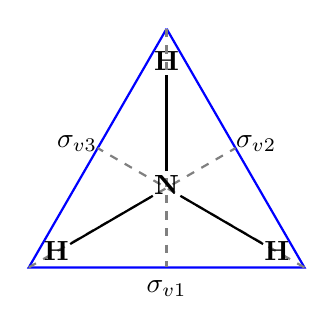
\begin{tikzpicture}[scale=1.75]
                        \coordinate (one) at (0,1.732);
                        \coordinate (two) at (1,0);
                        \coordinate (three) at (-1,0);
                        \coordinate (onetwo) at (0.5,0.866);
                        \coordinate (twothree) at (0,0);
                        \coordinate (onethree) at (-0.5,0.866);
                        \draw [blue,thick] (one)--(two)--(three)--(one);
                        \draw [gray,thick,dashed] (one)--(twothree);
                        \draw [gray,thick,dashed] (two)--(onethree);
                        \draw [gray,thick,dashed] (three)--(onetwo);
                        \draw [black,thick,solid] (0,0.7)--(0,1.4);
                        \draw [black,thick,solid] (-0.1,0.52)--(-0.7,0.17);
                        \draw [black,thick,solid] (0.1,0.52)--(0.7,0.17);
                        \node at (0,-0.15) {$\sigma_{v1}$};
                        \node at (0.65,0.9) {$\sigma_{v2}$};
                        \node at (-0.65,0.9)
                        {$\sigma_{v3}$};
                        \node at (0,0.6) {\textbf N};
                        \node at (0,1.5) {\textbf H};
                        \node at (-0.8,0.12) {\textbf H};
                        \node at (0.8,0.12) {\textbf H};
                    \end{tikzpicture}\\
                    \begin{tabular}{l}
                        $E$: Identity\\
                        $C_3$: $120^{\circ}$, CCW\\
                        $C_3^2$: $240^{\circ}$, CCW
                    \end{tabular}
                \end{tabular}
                &
                \begin{tabular}{cc|cccccc}
                    & & \multicolumn{6}{c}{$g$}\\
                    & $f \circ g$ & $E$ & $C_3$ & $C_3^2$ & $\sigma_{v1}$ & $\sigma_{v2}$ & $\sigma_{v3}$\\
                    \hline
                    \multirow{6}{*}{$f$} & $E$ & $E$ & $C_3$ & $C_3^2$ & $\sigma_{v1}$ & $\sigma_{v2}$ & $\sigma_{v3}$\\
                    & $C_3$ & $C_3$ & $C_3^2$ & $E$ & $\sigma_{v3}$ & $\sigma_{v1}$ & $\sigma_{v2}$\\
                    & $C_3^2$ & $C_3^2$ & $E$ & $C_3$ & $\sigma_{v2}$ & $\sigma_{v3}$ & $\sigma_{v1}$\\
                    & $\sigma_{v1}$ & $\sigma_{v1}$ & $\sigma_{v2}$ & $\sigma_{v3}$ & $E$ & $C_3$ & $C_3^2$\\
                    & $\sigma_{v2}$ & $\sigma_{v2}$ & $\sigma_{v3}$ & $\sigma_{v1}$ & $C_3^2$ & $E$ & $C_3$\\
                    & $\sigma_{v3}$ & $\sigma_{v3}$ & $\sigma_{v1}$ & $\sigma_{v2}$ & $C_3$ & $C_3^2$ & $E$
                \end{tabular}
            \end{tabular}
        \end{table}
    \end{frame}

    \begin{frame}{Algebraic group structure of point groups}
        We will do the same process with $C_{2v}$.
        \vs
        
        Clearly, $C_{2v}$ has an identity element $E$. The elements $C_2$, $\sigma_{v1}$, and $\sigma_{v2}$ are their own inverses. There are $4$ symmetry operations in $C_{2v}$: $\{E, C_2, \sigma_{v1}, \sigma_{v2}\}$.
        \vs
        
        Closure can be verified from the Cayley table, and associativity follows from the associativity of function composition.
        \vs
        
        Furthermore, from the Cayley table, we can see that $C_{2v}\cong V_4$.
    \end{frame}

    \begin{frame}{Algebraic group structure of point groups}
        \begin{table}[ht]
            \centering
            \renewcommand{\arraystretch}{1.5}
            \begin{tabular}{lcr}
                \begin{tabular}{l}
                    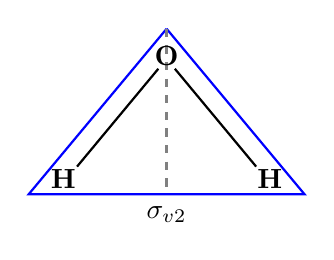
\begin{tikzpicture}[scale=1.75]
                        \coordinate (one) at (0,1.2);
                        \coordinate (two) at (1,0);
                        \coordinate (three) at (-1,0);
                        \coordinate (onetwo) at (0.5,0.866);
                        \coordinate (twothree) at (0,0);
                        \coordinate (onethree) at (-0.5,0.866);
                        \draw [blue,thick] (one)--(two)--(three)--(one);
                        \draw [gray,thick,dashed] (one)--(twothree);
                        \draw [black,thick,solid] (-0.06,0.91)--(-0.65,0.2);
                        \draw [black,thick,solid] (0.06,0.91)--(0.65,0.2);
                        \node at (0,-0.15) {$\sigma_{v2}$};
                        \node at (0,1) {\textbf O};
                        \node at (-0.75,0.11)
                        {\textbf H};
                        \node at (0.75,0.11)
                        {\textbf H};
                    \end{tikzpicture}\\
                    \begin{tabular}{l}
                        $E$: Identity\\
                        $C_2$: $180^{\circ}$\\
                        $\sigma_{v1}$: Refl. over molecular plane
                    \end{tabular}
                \end{tabular}
                &
                \begin{tabular}{cc|cccc}
                    & & \multicolumn{4}{c}{$g$}\\
                    & $f \circ g$ & $E$ & $C_2$ & $\sigma_{v1}$ & $\sigma_{v2}$\\
                    \hline
                    \multirow{4}{*}{$f$} & $E$ & $E$ & $C_2$ & $\sigma_{v1}$ & $\sigma_{v2}$\\
                    & $C_2$ & $C_2$ & $E$ & $\sigma_{v2}$ & $\sigma_{v1}$\\
                    & $\sigma_{v1}$ & $\sigma_{v1}$ & $\sigma_{v2}$ & $E$ & $C_2$\\
                    & $\sigma_{v2}$ & $\sigma_{v2}$ & $\sigma_{v1}$ & $C_2$ & $E$
                \end{tabular}
            \end{tabular}
        \end{table}
    \end{frame}

    \begin{frame}{Representation of symmetry operations as matrices}
        Now we find matrix representations of $E$, $C_n$, $\sigma$, $i$, and $S_n$. We will define these operations as transformations of the coordinate vector $(x,y,z)^T$.
        \vs

        \onslide<2->{
            The identity operation $E$ is represented by the identity matrix \[M_E=\begin{pmatrix}1&0&0\\0&1&0\\0&0&1\end{pmatrix}.\]
        }
        
        \onslide<3>{
            The rotation operation $C_n$, where the rotation is about the $z$ axis, is represented by the matrix \[M_{C_n}=\begin{pmatrix}\cos\theta&-\sin\theta&0\\\sin\theta&\cos\theta&0\\0&0&1\end{pmatrix},\] where $\theta=\dfrac{360^\circ}{n}$. Matrices for other axes can be constructed similarly.
        }
    \end{frame}
        
    \begin{frame}{Representation of symmetry operations as matrices}
        The reflection operations $\sigma$ over the $xy$, $yz$, and $xz$ planes are represented by the respective matrices \[M_{\sigma_{xy}}=\begin{pmatrix}1&0&0\\0&1&0\\0&0&-1\end{pmatrix}, M_{\sigma_{yz}}=\begin{pmatrix}-1&0&0\\0&1&0\\0&0&1\end{pmatrix}, \text{ and }M_{\sigma_{xz}}=\begin{pmatrix}1&0&0\\0&-1&0\\0&0&1\end{pmatrix}.\]
        
        \onslide<2->{
            The inversion operation $i$ is represented by the matrix \[M_i=\begin{pmatrix}-1&0&0\\0&-1&0\\0&0&-1\end{pmatrix}.\]
        }
        
        \onslide<3>{
            Finally, the rotation-reflection operation $S_n$ is represented by a matrix like \[M_{S_n}=\begin{pmatrix}\cos\theta&-\sin\theta&0\\\sin\theta&\cos\theta&0\\0&0&-1\end{pmatrix}.\]
        }
    \end{frame}

    \begin{frame}{Matrix representation of $C_{2v}$}
        We will look at the matrix representation for $C_{2v}$ (\ch{H2O}) first. We use the notation previously established in the Cayley table. By convention, we define the $z$ axis as the principal axis and the $xz$ plane as the plane of the molecule, with the oxygen atom at the origin, as shown:

        \begin{center}\includegraphics[width=1.5in]{waterxyz.png}\end{center}
    \end{frame}

    \begin{frame}{Matrix representation of $C_{2v}$}
        The matrices for the symmetry operations of $C_{2v}$ are \[M_E=\begin{pmatrix}1&0&0\\0&1&0\\0&0&1\end{pmatrix}, M_{C_2}=\begin{pmatrix}-1&0&0\\0&-1&0\\0&0&1\end{pmatrix},\]
        \[M_{\sigma_{v1}}=\begin{pmatrix}1&0&0\\0&-1&0\\0&0&1\end{pmatrix}, \text{ and } M_{\sigma_{v2}}=\begin{pmatrix}-1&0&0\\0&1&0\\0&0&1\end{pmatrix}.\] Multiplying these matrices reveals the same group structure as shown in the Cayley table.
    \end{frame}

    \begin{frame}{Matrix representation of $C_{3v}$}
        Now we will look at the matrix representation for $C_{3v}$ (\ch{NH3}). We use the notation previous established in the Cayley table. By convention, we define the $z$ axis as the principal axis, the $xy$ plane as parallel to the hydrogen triangle, and the $xz$ plane coinciding with one of the three $\sigma_v$ mirror planes, with the nitrogen atom at the origin, as shown:
        
        \begin{center}\includegraphics[width=1.5in]{ammoniaxyz.png}\end{center}
    \end{frame}

    \begin{frame}{Matrix representation of $C_{3v}$}
        The matrices for the symmetry operations of $C_{3v}$ are \[M_E=\begin{pmatrix}1&0&0\\0&1&0\\0&0&1\end{pmatrix}, M_{C_3}=\begin{pmatrix}-\frac12&-\frac{\sqrt{3}}2&0\\\frac{\sqrt{3}}2&-\frac12&0\\0&0&1\end{pmatrix},\]
        \[M_{C_3^2}=\begin{pmatrix}-\frac12&\frac{\sqrt{3}}2&0\\-\frac{\sqrt{3}}2&-\frac12&0\\0&0&1\end{pmatrix}, M_{\sigma_{v1}}=\begin{pmatrix}1&0&0\\0&-1&0\\0&0&1\end{pmatrix},\]
        \[M_{\sigma_{v2}}=\begin{pmatrix}-\frac12&-\frac{\sqrt{3}}2&0\\-\frac{\sqrt3}2&\frac12&0\\0&0&1\end{pmatrix}, \text{ and } M_{\sigma_{v3}}=\begin{pmatrix}-\frac12&\frac{\sqrt{3}}2&0\\\frac{\sqrt3}2&\frac12&0\\0&0&1\end{pmatrix}.\]
        
        Multiplying these matrices reveals the same group structure as shown in the Cayley table.
    \end{frame}

    \begin{frame}{Characters and reducible/irreducible representations}
        Constructing those matrices was challenging, especially in the case of $C_{3v}$, mainly because appropriate bases needed to be chosen, and the symmetries with respect to those bases needed to be computed with tedious hand calculations. Of course, different bases could have been used, which makes the matrix representations non-unique.
        \vs
        
        \onslide<2->{
            These problems are disappointing, especially considering that $C_{2v}$ and $C_{3v}$ are two of the simplest and most common point groups in chemistry!
            \vs
        }

        \onslide<3> {
            Thankfully, we have that the trace (character) of a matrix is conjugation invariant. Thus, if we change the basis, the characters remain the same.
        }
    \end{frame}

    \begin{frame}{Characters and reducible/irreducible representations}
        To simplify the representations, we will use characters instead of matrices. The characters in $C_{2v}$ are $\chi_E = 3$, $\chi_{C_2}=-1$, $\chi_{\sigma_{v1}}=1$, and $\chi_{\sigma_{v2}}=1$. The characters in $C_{3v}$ are $\chi_E=3$, $\chi_{C_3}=0$, $\chi_{C_3^2}=0$, $\chi_{\sigma_{v1}}=1$, $\chi_{\sigma_{v2}}1$, and $\chi_{\sigma_{v3}}=1$.
        \vs

        \onslide<2->{
            The conjugacy classes in $C_{2v}$ are the singletons $\{E\}, \{C_2\}, \{\sigma_{v1}\},$ and $\{\sigma_{v2}\}$, which follows since $C_{2v}\cong V_4$ is an abelian group. The conjugacy classes in $C_{3v}$ are the sets $\{E\}, \{C_3,C_3^2\},$ and $\{\sigma_{v1},\sigma_{v2},\sigma_{v3}\}$. Every operation in the same class has the same character, so they will be grouped together in the character tables.
            \vs
        }

        \onslide<3>{
            The characters listed above for $C_{2v}$ and $C_{3v}$ are reducible representations. We will denote reducible representations by $\Gamma$. Our goal is to decompose these reducible representations into irreducible representations (\emph{irreps}).
        }
    \end{frame}

    \begin{frame}{Irrep notation crash course}
        The irreps will be denoted using a standard notation system.
        \vs

        One dimensional irreps are denoted $A$ if the representation is symmetric to the principal rotation (that is, $\chi_{C_n}=1$) and $B$ if the representation is antisymmetric to the principal rotation ($\chi_{C_n}=-1$).
        \vs
        
        Two dimensional irreps are denoted $E$, and three dimensional irreps are denoted $T$.
        \vs
        
        Furthermore, subscripts are used to distinguish irreps with the same dimension. Subscript 1 is used for an irrep that is symmetric to a perpendicular $C_2$ axis, and subscript 2 is used for an irrep that is antisymmetric to a perpendicular $C_2$. If there is no perpendicular $C_2$ axis, the subscript is determined based on the symmetry (1) or antisymmetry (2) with respect to the vertical mirror plane $xz$.
    \end{frame}

    \begin{frame}{Character tables}
        We now construct the character table of $C_{2v}$. We block diagonalize the matrices we had before: \[M_E=\begin{pmatrix}\boxed1&0&0\\0&\boxed1&0\\0&0&\boxed1\end{pmatrix}, M_{C_2}=\begin{pmatrix}\boxed{-1}&0&0\\0&\boxed{-1}&0\\0&0&\boxed1\end{pmatrix},\]
        \[M_{\sigma_{v1}}=\begin{pmatrix}\boxed1&0&0\\0&\boxed{-1}&0\\0&0&\boxed1\end{pmatrix}, \text{ and } M_{\sigma_{v2}}=\begin{pmatrix}\boxed{-1}&0&0\\0&\boxed1&0\\0&0&\boxed1\end{pmatrix}.\]
    \end{frame}

    \begin{frame}{Character tables}
        We place the elements from the first block in the first row ($x$), the elements from the second block in the second row ($y$), and the elements from the third block in the third row ($z$), and labeling the rows by the aforementioned rules. The last two columns and the empty row will be filled in later.

        \begin{table}[h]
            \centering
            \renewcommand{\arraystretch}{1.5}
            \begin{tabular}{c|cccc|c|c}
                $C_{2v}$ & $E$ & $C_2$ & $\sigma_{v1}~(xz)$ & $\sigma_{v2}~(yz)$ & ~~~~~~~ & ~~~~~~~\\
                \hline
                $B_1$ & 1 & -1 & 1 & -1 & $x$ &\\
                $B_2$ & 1 & -1 & -1 & 1 & $y$ &\\
                $A_1$ & 1 & 1 & 1 & 1 & $z$ &\\
                &&&&&&\\
                \hline
                $\Gamma$ & 3 & -1 & 1 & 1 & &
            \end{tabular}
        \end{table}
    \end{frame}

    \begin{frame}{Character tables}
        Character tables have several important properties. Let $\chi_i(C)$ represent the character of class $C$ in the $i$th irrep.
        \vs
        
        \begin{itemize}
            \item The number of symmetry operations is the order of the group, $h$.
            \item If symmetry operations are grouped by conjugacy class $C$, we show how many operations are in the class, $n_C$, in the top row. For example, if there are three rotations in the $C_2$ class, the top row will be labeled $3C_2$. We will call $n_C$ the multiplicity of the class.
            \item The number of irreps equals the number of classes. That is, the character table needs to have the same number of rows and columns.
            \item Taking the sum over all of the irreps, we have \[\sum_i\chi_i^2(E)=h,\] where $E$ is the identity operation.
        \end{itemize}
    \end{frame}

    \begin{frame}{Character tables}
        \begin{itemize}
            \item For the $i$th irrep, we have \begin{equation}\sum_C n_C \chi_i^2(C)=h,\label{sumsq}\end{equation} where the sum is taken over all of the conjugacy classes.
            \item \textbf{Orthogonality Theorem.} Irreps are orthogonal. We have, for the $i$th and $j$th irreps, \begin{equation}
            \sum_C n_C \chi_i(C)\chi_j(C)=h\delta_{ij},\label{orthog}\end{equation} where $\delta_{ij}$ is the Kronecker delta. When $i=j$, \eqref{orthog} reduces to \eqref{sumsq}, and when $i\neq j$, we have \[\sum_C n_C \chi_i(C)\chi_j(C)=0.\] 
            \item One irrep has characters that are all $1$, which is labeled $A_1$.
            \item Each irrep must be distinct.
        \end{itemize}
    \end{frame}

    \begin{frame}{Character tables}
        Applying these rules, we deduce that there is indeed a fourth irrep, and using the Orthogonality Theorem along with the other properties, we can find the characters of this fourth irrep, $A_2$.

        \begin{table}[h]
            \centering
            \renewcommand{\arraystretch}{1.5}
            \begin{tabular}{c|cccc|c|c}
                $C_{2v}$ & $E$ & $C_2$ & $\sigma_{v1}~(xz)$ & $\sigma_{v2}~(yz)$ & &\\
                \hline
                $A_1$ & 1 & 1 & 1 & 1 & $z$ & $x^2, y^2, z^2$\\
                $A_2$ & 1 & 1 & -1 & -1 & $R_z$ & $xy$\\
                $B_1$ & 1 & -1 & 1 & -1 & $x, R_y$ & $xz$\\
                $B_2$ & 1 & -1 & -1 & 1 & $y, R_x$ & $yz$\\
            \end{tabular}
        \end{table}

        We now have a complete character table for $C_{2v}$. Additional information has been added to the last two columns. $R_x$, $R_y$, and $R_z$ indicate the irreps that match the symmetry of rotations about the $x$, $y$, and $z$ axes, respectively. $x^2$, $y^2$, $xy$, etc. represent functions that are symmetric with respect to the irreps. To save time, we will omit some details.
    \end{frame}

    \begin{frame}{Character tables}
        We now construct the character table for $C_{3v}$. We block diagonalize the matrices we had before: \[M_E=\left(\begin{array}{cc|c}1&0&0\\0&1&0\\\hline0&0&1\end{array}\right), M_{C_3}=\left(\begin{array}{cc|c}-\frac12&-\frac{\sqrt{3}}2&0\\\frac{\sqrt{3}}2&-\frac12&0\\\hline0&0&1\end{array}\right),\]
        \[M_{C_3^2}=\left(\begin{array}{cc|c}-\frac12&\frac{\sqrt{3}}2&0\\-\frac{\sqrt{3}}2&-\frac12&0\\\hline0&0&1\end{array}\right), M_{\sigma_{v1}}=\left(\begin{array}{cc|c}1&0&0\\0&-1&0\\\hline0&0&1\end{array}\right)\]
        \[M_{\sigma_{v2}}=\left(\begin{array}{cc|c}-\frac12&-\frac{\sqrt{3}}2&0\\-\frac{\sqrt3}2&\frac12&0\\\hline0&0&1\end{array}\right), \text{ and } M_{\sigma_{v3}}=\left(\begin{array}{cc|c}-\frac12&\frac{\sqrt{3}}2&0\\\frac{\sqrt3}2&\frac12&0\\\hline0&0&1\end{array}\right).\]
    \end{frame}

    \begin{frame}{Character tables}
        The $C_3$ and $C_3^2$ operations are in the same class, and likewise the three $\sigma_v$ operations are in the same class, so they will be grouped together.
        \vs

        Following the above procedure established, we create the full character table for $C_{3v}$.
    
        \begin{table}[h]
            \centering
            \renewcommand{\arraystretch}{1.5}
            \begin{tabular}{c|ccc|c|c}
                $C_{3v}$ & $E$ & $2C_3$ & $3\sigma_{v}$ & &\\
                \hline
                $A_1$ & 1 & 1 & 1 & $z$ & $x^2+y^2, z^2$\\
                $A_2$ & 1 & 1 & -1 & $R_z$ &\\
                $E$ & 2 & -1 & 0 & $(x,y), (R_x,R_y)$ & $(x^2-y^2,xy),(xz,yz)$\\
            \end{tabular}
        \end{table}
        We can verify that the order and orthogonality relations hold. Also, notice that we group $x$ and $y$ together in parentheses. This is based on the block diagonalization, where $x$ and $y$ together form one block and $z$ individually forms another block.
    \end{frame}

    \begin{frame}{Expressing reducible representations in terms of irreps}
        The reducible representation $\Gamma$ can be written as a linear combination of the irreps. That is, for each class $C$, and for each character $\chi(C)$ in $\Gamma$, with corresponding character $\chi_i(C)$ in the $i$th irrep, there exist coefficients $n_1, n_2,\ldots$ such that \begin{equation}\chi_C=\sum_in_i\chi_i(C).\label{lincomb}\end{equation}
        \vs
        
        \textbf{Lemma 1.} Each coefficient $n_i$ in \eqref{lincomb} is given by
        \[n_i=\frac1h\sum_Cn_C\chi(C)\chi_i(C),\]
        where $h$ is the order of the group.
        \vs

        We can use this to find the number of times that an irrep contributes to $\Gamma$. We will look at an application in the next section, where we consider the vibrations of the water molecule.
    \end{frame}

    \begin{frame}{Expressing reducible representations in terms of irreps}
        \begin{proof}
            From the Orthogonality Theorem, we have, for the $i$th and $j$th irreps, \[\sum_C n_C \chi_i(C)\chi_j(C)=h\delta_{ij}.\]
            Taking the sum over all $j$ irreps, and multiplying both sides by $n_j$, we have \begin{equation}\sum_C n_C\sum_jn_j \chi_i(C)\chi_j(C)=h\sum_jn_j\delta_{ij}=hn_i.\label{lemmastep2}\end{equation}
            We have by \eqref{lincomb} that $\sum_jn_j\chi_j(C)=\chi(C)$. Substituting into \eqref{lemmastep2}, we get \[\sum_C n_C\chi(C)\chi_i(C)=hn_i.\] Divide both sides by $h$ to complete the proof.
        \end{proof}
    \end{frame}

    \begin{frame}{Molecular vibrations}
        Individual atoms can move slightly within a molecule. To study the vibrations within the water molecule, we first assign a 3D coordinate axis to each atom. For convenience, we stick with the same layout that we previously used for water. This time, however, each atom can be considered to be at its own origin.
        \vs

        For a molecule with $N$ atoms, each atom can move in three dimensions, so there are $3N$ \emph{degrees of freedom}. Hence, water has nine degrees of freedom, three for each atom.
        \vs

        In a nonlinear molecule, there are three translational \emph{modes}, three rotational modes, and the remaining $3N-6$ modes are vibrational. In a linear molecule, there are also three translational modes. However, a linear molecule only has two rotational modes, since a rotation along the axis of the molecule does not change the relative orientation of the atoms. Then the remaining $3N-5$ modes are vibrational.
    \end{frame}

    \begin{frame}{Molecular vibrations}
        Since water is bent (nonlinear), it has $3N-6=3$ vibrational modes. One of these is \emph{symmetric stretch}, where the lengths of the \ch{O-H} bonds lengthen and shorten in unison. One is \emph{antisymmetric stretch}, where one \ch{O-H} bond lengthens as the other one shortens. The last one is \emph{symmetric bend}, where the bond angle increases and decreases, similar to a bird flapping its wings. Each of these vibrational modes changes the \emph{dipole moment} of water, causing its polarity to oscillate slightly.
        \vs
        
        \url{https://www.chem.purdue.edu/jmol/vibs/h2o.html}
    \end{frame}

    \begin{frame}{Molecular vibrations}
        If we create a $9\times9$ matrix to represent the effect of a symmetry operation on the position of each atom in the water molecule, an element in the diagonal of the matrix will be 1 if the atom remains in its original location, -1 if it reverses direction, and 0 if it moves. We can then take the character of the matrix for each symmetry operation. Since operations in the same class have the same character, we only need to construct one such matrix for each class.
        \vs
        
        However, actually creating such large matrices for each class is rather tedious. Thankfully, we can speed through the process by thinking carefully about each symmetry operation.
    \end{frame}

    \begin{frame}{Molecular vibrations}
        In the identity operation $E$, every atom remains in the same position, so $\chi_E=9$. In the rotation $C_2$, the hydrogen atoms both move, so they contribute nothing to the character. The oxygen atom reverses direction with respect to $x$ $(-1)$ and $y$ $(-1)$, but not with respect to $z$ $(1)$. Thus, oxygen contributes a net of $-1$ to the character. Hence $\chi_{C_2}=-1$. In the reflection $\sigma_{v1}~(xz)$, in the plane of the molecule, the $x$ and $z$ directions stay the same for each atom, while the $y$ direction flips for each atom. Then $\chi_{\sigma_{v1}}=3-3+3=3$. In the reflection $\sigma_{v2}~(yz)$, the hydrogen atoms swap positions, so they contribute nothing to the character. The oxygen atom reverses direction with respect to $x$ $(-1)$ but not with respect to $y$ $(1)$ or $z$ $(1)$. Therefore, $\chi_{\sigma_{v2}}=1$. We are now ready to show the full $C_{2v}$ character table again, this time with $\Gamma$ included.
    \end{frame}

    \begin{frame}{Molecular vibrations}
        \begin{table}[h]
            \centering
            \renewcommand{\arraystretch}{1.5}
            \begin{tabular}{c|cccc|c|c}
                $C_{2v}$ & $E$ & $C_2$ & $\sigma_{v1}$ & $\sigma_{v2}$ & &\\
                \hline
                $A_1$ & 1 & 1 & 1 & 1 & $z$ & $x^2, y^2, z^2$\\
                $A_2$ & 1 & 1 & -1 & -1 & $R_z$ & $xy$\\
                $B_1$ & 1 & -1 & 1 & -1 & $x, R_y$ & $xz$\\
                $B_2$ & 1 & -1 & -1 & 1 & $y, R_x$ & $yz$\\
                \hline
                $\Gamma$ & 9 & -1 & 3 & 1 & &\\
            \end{tabular}
        \end{table}

        We can now use Lemma 1 to express $\Gamma$ as a linear combination of the irreps $A_1, A_2, B_1$, and $B_2$. We have \[n_{A_1}=\frac14((9)(1)+(-1)(1)+(3)(1)+(1)(1))=3.\] Similarly, we calculate $n_{A_2}=1$, $n_{B_1}=3$, and $n_{B_2}=2$. We find that \begin{equation}\Gamma = 3A_1+A_2+3B_1+2B_2.\label{linearcombo}\end{equation}
    \end{frame}
    
    \begin{frame}{Molecular vibrations}
        Looking at the character table, the three translational modes of a $C_{2v}$ molecule correspond to the irreps that have $x$, $y$, or $z$ listed on the right hand side, which are $A_1$, $B_1$, and $B_2$. The three rotational modes correspond to the irreps that have $R_x$, $R_y$ and $R_z$ listed, which are $A_2$, $B_1$, and $B_2$. Taking \eqref{linearcombo} and subtracting $A_1 + B_1 + B_2 + A_2 + B_1 + B_2$, for the translational and rotational modes, we have $2A_1+B_1$ remaining, which are the three vibrational modes. Two correspond to the $A_1$ irrep and one corresponds to the $B_1$ irrep.
    \end{frame}

    \begin{frame}{Applications: Spectroscopy}
        Much information can be determined about a molecule based on how it absorbs infrared light at various wavelengths. IR spectroscopy is a very common technique to ``draw a picture'' of a molecule in order to learn about the bonds and groups of atoms present. Below, we see a labeled IR spectrum of water. \cite{gutow2015}

        \begin{center}
            \includegraphics[width=4.5in]{irwater.png}
        \end{center}
    \end{frame}

    \begin{frame}{Applications: Spectroscopy}
        When a molecule absorbs IR light, vibrations that result in a change of dipole moment are affected. As we said earlier, the three vibrational modes of water all impact the dipole moment of water, so they appear in the IR spectrum. (The two stretch bands are so close together and broad that they merge into one large peak.)
        \vs
        
        Interestingly, even though carbon dioxide (\ch{CO2}) is nonpolar by linear symmetry, when it absorbs infrared light, it will vibrate in such a way as to momentarily break the linear symmetry and make \ch{CO2} slightly polar! This is why \ch{CO2} absorbs infrared light, making it a greenhouse gas. \cite{royal2009}
    \end{frame}

    \begin{frame}{Applications: Spectroscopy}
        How do we know which vibrational modes are \emph{IR active}? We look at the character table and see which irreps have the same symmetry as $x$, $y$, or $z$. In the last section, we determined that water has two vibrational modes corresponding to the irrep $A_1$ and one corresponding to the irrep $B_1$. We see that $A_1$ has the same symmetry as $z$ and $B_1$ has the same symmetry as $x$, so all three vibrational modes of water are IR active. This makes sense, since we said earlier that each of the vibrational modes of water changes the dipole moment!
        \vs
        
        If there were a vibrational mode corresponding to, say, the $A_2$ irrep, then that mode would be \emph{IR inactive} and not appear on an IR spectrum. But we have mathematically eliminated that possibility for water.
    \end{frame}

    \begin{frame}{Applications: Spectroscopy}
        With Raman spectroscopy, high energy light bombards molecules, putting them into an excited state. When they relax back to their various vibrational energy states, they release radiation that can be detected. A vibrational mode is \emph{Raman active} if it exhibits a change of polarizability, which is the tendency to acquire a dipole moment from an electric field. To determine which vibrational modes are Raman active, we look for those irreps that have the same symmetry as $x^2$, $y^2$, $z^2$, $xy$, $yz$, or $xz$, or a linear combination of those. All of the vibrational modes of water are Raman active, which we can determine quickly from the $C_{2v}$ character table.
    \end{frame}

    \begin{frame}{Applications: Chirality \cite{monash}}
        Our hands are mirror images of each other, but they are not superimposable. Likewise, \emph{chiral} molecules are those that are non-superimposable over their mirror images. When an atom is bonded to four distinct atoms or clusters of atoms, the molecule is chiral. Each configuration is called an \emph{enantiomer}. A non-chiral molecule is \emph{achiral}.

        \begin{center}\includegraphics[width=2.5in]{enantiomers.png}\end{center}

        Notice that it is impossible to rotate the molecule on the left to look exactly like the molecule on the right.
    \end{frame}

    \begin{frame}{Applications: Chirality \cite{halpern}}
        Chiral compounds may occur in \emph{racemic mixtures}, 50/50 mixtures of enantiomers. However, if plane polarized light is passed through a substance consisting of an unequal balance of the enantiomers, the direction of the light will rotate. This is called \emph{optical activity}. The two enantiomers rotate light in opposite directions. This is the principle behind how liquid crystal displays (LCDs) work! \cite{lininger2022}

        \begin{center}
            \includegraphics[width=3in]{chiral.jpg}
        \end{center}
    \end{frame}

    \begin{frame}{Applications: Chirality}
        Interestingly, ibuprofen is a chiral molecule. It is sold as a racemic mixture, although only one of its enantiomers is effective. Furthermore, the drug thalidomide is chiral. One of its enantiomers is a sedative, while the other causes extreme birth defects. \cite{jonsson2017}
        \vs

        If a molecule contains any $\sigma$, $S_n$, or $i$ symmetry elements, it is achiral. Hence, the only symmetries possible for a chiral compound are the identity $E$ and proper rotation axes $C_n$. A look at the character table of a molecule's point group will tell which symmetry elements are present, from which one can deduce if the molecule may be chiral.
    \end{frame}

    \begin{frame}[allowframebreaks]{References}
        \printbibliography
    \end{frame}
\end{document}